\documentclass{article}
\usepackage{amsmath}
\usepackage{amssymb}
\usepackage{amsthm}
\usepackage{amsfonts}
\usepackage[margin=2cm]{geometry}
\usepackage{graphicx}
\usepackage{color}
\usepackage[all]{xy}
\newtheorem*{lem}{Lemma}

\title{Solution for Exercise sheet 6}
\author{Yikai Teng, You Zhou}
\date{Exercise session: Thu. 8-10}

\begin{document}
\maketitle
\paragraph{Exercise 6.1}We first show that $m=n+k.$ Every point $b\in S^n$ has a small neighborhood $U$ that is homeomorphic to $\mathbb{R}^n.$ Since $p$ is a fiber bundle, we may assume that $p^{-1}(U)\cong U\times S^k\cong\mathbb{R}^n\times S^k.$ A point $x\in\mathbb{R}^n\times S^k$ then has a neighborhood homeomorphic to $\mathbb{R}^n\times\mathbb{R}^k$ and such that its inverse image under the homeomorphism $p^{-1}(U)\xrightarrow{\cong}\mathbb{R}^n\times S^k$ is homeomorphic to $\mathbb{R}^m.$ This shows that $m=n+k.$

We then show that $k=n-1.$ If $m=1,$ then this follows from $m=n+k$ and $n\geq1.$ If $m=2,$ then either $n=2, k=0$ or $n=k=1.$ In the first case, $p$ is a two-fold covering map. But this is impossible since $\pi_1(S^2)=0$ and has no index-2 subgroup. In the second case, we have the long exact sequence
\[\cdots\rightarrow\pi_i(S^k)\rightarrow\pi_i(S^m)\rightarrow\pi_i(S^n)\rightarrow\pi_{i-1}(S^k)\rightarrow\cdots.\]
Since $\pi_2(S^1)=0,$ taking $n=2$ gives us an exact sequence $0\rightarrow\mathbb{Z}\rightarrow0,$ which is also impossible. When $m>2,$ still consider the exact sequence above. Then we have exact sequences
\[0\rightarrow\pi_i(S^n)\rightarrow\pi_{i-1}(S^k)\rightarrow0\]
for all $1<i<m.$ From this we get $n$ cannot be 1 since otherwise we would have $\pi_{k+1}(S^1)\rightarrow\pi_k(S^k)\rightarrow0$ exact. So $\pi_1(S^n)=0$ and there is a common $i$ that is the minimal $i$ such that $\pi_i(S^n)$ and $\pi_{i-1}(S^k)$ are not trivial. This shows that $k=n-1.$

\paragraph{Exercise 6.3}First note that there is a homeomorphism
\[\Omega X\times \Omega X\cong X^{(S^1\vee S^1, y_0)},\]
where $y_0$ is the point of intersection of the two circles. The map from the left side to the right side can be given by
\[\varphi\colon(f_1,f_2) \mapsto \left(x\mapsto f_i(x),  \text{ if } x\text{ is in the } i\text{-th wedge summand}\right)\]
and map in the opposite direction is
\[\psi\colon g\mapsto(g\circ i_1, g\circ i_2),\]
where $i_1,i_2$ are two wedge summand inclusions. By definition they are inverse to each other and are both continuous. (The continuity can be easily checked on subbasis.)

Let $\widetilde{\nabla^2}$ be $\nabla^2$ with the three vertices glued together and $q\colon \nabla^2\rightarrow\widetilde{\nabla^2}$ be the quotient map, then $q^*\colon X^{\widetilde{\nabla^2}}\rightarrow X^{\nabla^2}$ is a homeomorphism onto its image, which is just $E.$ So it suffices to show that the map
\[\Phi\colon X^{\widetilde{\nabla^2}}\rightarrow X^{S^1\vee S^1},\quad f\mapsto (f\circ i')\vee(f\circ j')\]
is a homotopy equivalence, where
\[i',j'\colon S^1\rightarrow\nabla^2\]
is defined by
\[i'(e^{2\pi it})=(t,1-t,0)\quad\text{respectively}\quad j'(e^{2\pi it})=(0,t,1-t)\]
and
\[(f\circ i')\vee(f\circ j')(x)=\begin{cases}
                                  f\circ i'(x), & \mbox{if } x\text{ is in the first wedge summand} \\
                                  f\circ j'(x), & \mbox{if } x\text{ is in the second wedge summand}.
                                \end{cases}.
\]

To prove this, we will first construct a homotopy equivalence between $\widetilde{\nabla^2}$ and $S^1\vee S^1$ whose induced map on mapping spaces is $\Phi$ and then show a general property that under certain assumptions, a homotopy equivalence map induces homotopy equivalence on mapping spaces. For the first step, to avoid messy notations and formulas, I express the maps $\alpha\colon\widetilde{\nabla^2}\rightarrow S^1\vee S^1$ and $\beta\colon S^1\vee S^1\rightarrow\widetilde{\nabla^2}$ in figures \ref{alpha} and \ref{beta} below. Then by definition $\alpha\circ\beta=\text{id}_{S^1\vee S^1}.$ Moreover, a homotopy equivalence from $\text{id}_{\widetilde{\nabla^2}}$ to $\beta\circ\alpha$ can also be constructed as illustrated in figure \ref{hmtp} below.
\begin{figure}[h]
  \centering
  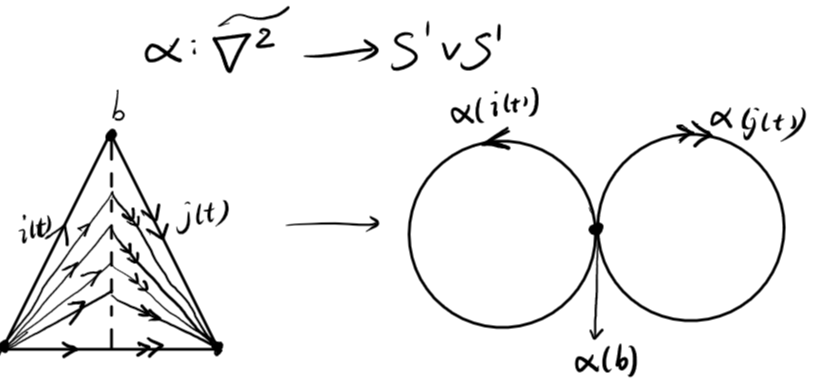
\includegraphics[width=9cm]{6.3_1}
  \caption{The map $\alpha$}\label{alpha}
\end{figure}

\begin{figure}[h]
  \centering
  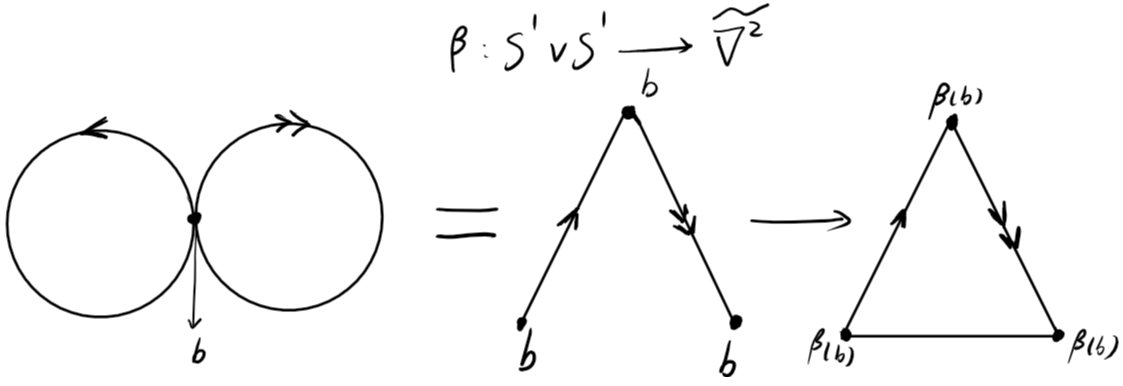
\includegraphics[width=9cm]{6.3_2}
  \caption{The map $\beta$}\label{beta}
\end{figure}

\begin{figure}[hb]
  \centering
  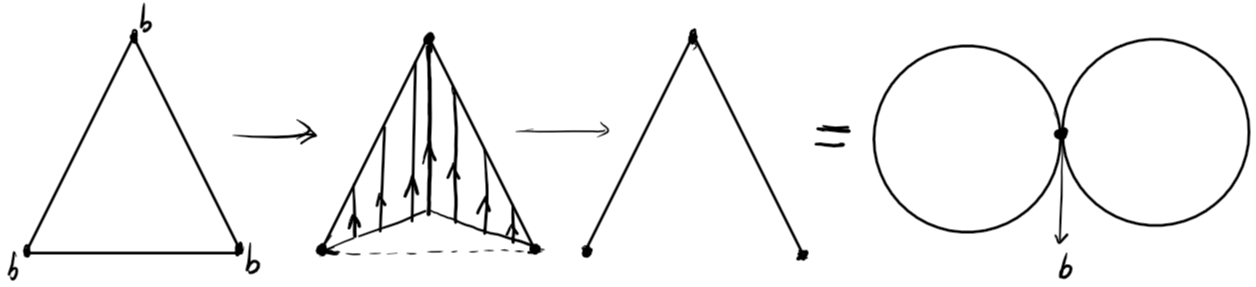
\includegraphics[width=9cm]{6.3_3}
  \caption{Homotopy between $\widetilde{\nabla^2}$ and $S^1\vee S^1$}\label{hmtp}
\end{figure}

So we have constructed our expected homotopy equivalence. By definition its induced map $\beta^*\colon X^{\widetilde{\nabla^2}}\rightarrow X^{S^1\vee S^1}$ is just $\Phi.$

Now we do the second step. Suppose that $X,Y$ and $Z$ are topological spaces,  $f\colon X\rightarrow Y$ is a homotopy equivalence and that $g\colon Y\rightarrow X$ is the homotopy inverse of $f$. We may assume that $X$ and $Y$ are both Hausdorff since $\widetilde{\nabla^2}$ and $S^1\vee S^1$ have this property. We have a continuous map
\[H\colon Y\times[0,1]\rightarrow Y\]
such that $H(y,0)=f\circ g(y)$ and $H(y,1)=y$ for all $y\in Y.$ Since $Y$ is Hausdorff,
\[H^*\colon Z^Y\times[0,1]\rightarrow Z^Y,\quad (h(\cdot),t)\mapsto (h(H(\cdot,t)))\]
is a continuous map that gives a homotopy between the identity and $(f\circ g)^*.$ Similarly, we can show that $(g\circ f)^*$ is also homotopy equivalent to the identity. Thus $f$ and $g$ really induce homotopy equivalence between mapping spaces $Z^X$ and $Z^Y.$ Combining these two steps then finishes our proof.
\end{document} 